% Options for packages loaded elsewhere
% Options for packages loaded elsewhere
\PassOptionsToPackage{unicode}{hyperref}
\PassOptionsToPackage{hyphens}{url}
\PassOptionsToPackage{dvipsnames,svgnames,x11names}{xcolor}
%
\documentclass[
  11pt,
  letterpaper,
]{article}
\usepackage{xcolor}
\usepackage[margin=0.78in]{geometry}
\usepackage{amsmath,amssymb}
\setcounter{secnumdepth}{-\maxdimen} % remove section numbering
\usepackage{iftex}
\ifPDFTeX
  \usepackage[T1]{fontenc}
  \usepackage[utf8]{inputenc}
  \usepackage{textcomp} % provide euro and other symbols
\else % if luatex or xetex
  \usepackage{unicode-math} % this also loads fontspec
  \defaultfontfeatures{Scale=MatchLowercase}
  \defaultfontfeatures[\rmfamily]{Ligatures=TeX,Scale=1}
\fi
\usepackage{lmodern}
\ifPDFTeX\else
  % xetex/luatex font selection
\fi
% Use upquote if available, for straight quotes in verbatim environments
\IfFileExists{upquote.sty}{\usepackage{upquote}}{}
\IfFileExists{microtype.sty}{% use microtype if available
  \usepackage[]{microtype}
  \UseMicrotypeSet[protrusion]{basicmath} % disable protrusion for tt fonts
}{}
\makeatletter
\@ifundefined{KOMAClassName}{% if non-KOMA class
  \IfFileExists{parskip.sty}{%
    \usepackage{parskip}
  }{% else
    \setlength{\parindent}{0pt}
    \setlength{\parskip}{6pt plus 2pt minus 1pt}}
}{% if KOMA class
  \KOMAoptions{parskip=half}}
\makeatother
% Make \paragraph and \subparagraph free-standing
\makeatletter
\ifx\paragraph\undefined\else
  \let\oldparagraph\paragraph
  \renewcommand{\paragraph}{
    \@ifstar
      \xxxParagraphStar
      \xxxParagraphNoStar
  }
  \newcommand{\xxxParagraphStar}[1]{\oldparagraph*{#1}\mbox{}}
  \newcommand{\xxxParagraphNoStar}[1]{\oldparagraph{#1}\mbox{}}
\fi
\ifx\subparagraph\undefined\else
  \let\oldsubparagraph\subparagraph
  \renewcommand{\subparagraph}{
    \@ifstar
      \xxxSubParagraphStar
      \xxxSubParagraphNoStar
  }
  \newcommand{\xxxSubParagraphStar}[1]{\oldsubparagraph*{#1}\mbox{}}
  \newcommand{\xxxSubParagraphNoStar}[1]{\oldsubparagraph{#1}\mbox{}}
\fi
\makeatother


\usepackage{longtable,booktabs,array}
\newcounter{none} % for unnumbered tables
\usepackage{calc} % for calculating minipage widths
% Correct order of tables after \paragraph or \subparagraph
\usepackage{etoolbox}
\makeatletter
\patchcmd\longtable{\par}{\if@noskipsec\mbox{}\fi\par}{}{}
\makeatother
% Allow footnotes in longtable head/foot
\IfFileExists{footnotehyper.sty}{\usepackage{footnotehyper}}{\usepackage{footnote}}
\makesavenoteenv{longtable}
\usepackage{graphicx}
\makeatletter
\newsavebox\pandoc@box
\newcommand*\pandocbounded[1]{% scales image to fit in text height/width
  \sbox\pandoc@box{#1}%
  \Gscale@div\@tempa{\textheight}{\dimexpr\ht\pandoc@box+\dp\pandoc@box\relax}%
  \Gscale@div\@tempb{\linewidth}{\wd\pandoc@box}%
  \ifdim\@tempb\p@<\@tempa\p@\let\@tempa\@tempb\fi% select the smaller of both
  \ifdim\@tempa\p@<\p@\scalebox{\@tempa}{\usebox\pandoc@box}%
  \else\usebox{\pandoc@box}%
  \fi%
}
% Set default figure placement to htbp
\def\fps@figure{htbp}
\makeatother





\setlength{\emergencystretch}{3em} % prevent overfull lines

\providecommand{\tightlist}{%
  \setlength{\itemsep}{0pt}\setlength{\parskip}{0pt}}



 


\usepackage{amsmath,amssymb}
\usepackage{fancyhdr}
\setlength{\headheight}{14pt}
\pagestyle{fancy}
\fancyhf{}
\renewcommand{\headrulewidth}{0pt}
\cfoot{\thepage}
\setlength{\parindent}{0pt}
\setlength{\parskip}{0.55em}
\makeatletter
\@ifpackageloaded{caption}{}{\usepackage{caption}}
\AtBeginDocument{%
\ifdefined\contentsname
  \renewcommand*\contentsname{Table of contents}
\else
  \newcommand\contentsname{Table of contents}
\fi
\ifdefined\listfigurename
  \renewcommand*\listfigurename{List of Figures}
\else
  \newcommand\listfigurename{List of Figures}
\fi
\ifdefined\listtablename
  \renewcommand*\listtablename{List of Tables}
\else
  \newcommand\listtablename{List of Tables}
\fi
\ifdefined\figurename
  \renewcommand*\figurename{Figure}
\else
  \newcommand\figurename{Figure}
\fi
\ifdefined\tablename
  \renewcommand*\tablename{Table}
\else
  \newcommand\tablename{Table}
\fi
}
\@ifpackageloaded{float}{}{\usepackage{float}}
\floatstyle{ruled}
\@ifundefined{c@chapter}{\newfloat{codelisting}{h}{lop}}{\newfloat{codelisting}{h}{lop}[chapter]}
\floatname{codelisting}{Listing}
\newcommand*\listoflistings{\listof{codelisting}{List of Listings}}
\makeatother
\makeatletter
\makeatother
\makeatletter
\@ifpackageloaded{caption}{}{\usepackage{caption}}
\@ifpackageloaded{subcaption}{}{\usepackage{subcaption}}
\makeatother
\usepackage{bookmark}
\IfFileExists{xurl.sty}{\usepackage{xurl}}{} % add URL line breaks if available
\urlstyle{same}
% fallback for those not using the hyperref driver hyperxmp:
\makeatletter
\@ifundefined{xmpquote}{\newcommand{\xmpquote}[1]{#1}}{}
\makeatother
\hypersetup{
  colorlinks=true,
  linkcolor={blue},
  filecolor={Maroon},
  citecolor={Blue},
  urlcolor={Blue},
  pdfcreator={LaTeX via pandoc}}


\author{}
\date{}
\begin{document}


\begin{center}
{\LARGE Exam 1, Fall 2021}\\[1.2em]
Date: \rule{1.6in}{0.4pt}
\end{center}

\vspace{2.3em}

First name:

\rule{2.05in}{0.4pt}

\hfill Last name:

\rule{2.05in}{0.4pt}

\vspace{2.2em}

\textbf{HONOR STATEMENT:} I have neither given nor received aid on this
examination.

\vspace{2em}

Signature:

\rule{5.2in}{0.4pt}

\vspace{2.5em}

This is a closed-book, closed-note exam. Calculators or other electronic
devices are not allowed. Note that throughout the exam, full credit is
given even when calculations are fully outlined but not complete,
i.e.~\(\displaystyle \frac{\frac{1}{2}\times 4+\frac{8}{4}}{2}\)
receives the same credit as an answer of 2.

\vspace{2em}

Possibly helpful equations:

If \(X\) is a binomial random variable, its distribution is given by

\[
P(X=x)=\binom{n}{x}\pi^x(1-\pi)^{n-x},
\]

where \(\pi\) is the probability of success, and \(n\) is the number of
independent trials.

\vspace{1.5em}

For events \(A\) and \(B\), Bayes' theorem tells us

\[
P(A\mid B)=\frac{P(B\mid A)P(A)}{P(B)}=\frac{P(B\cap A)}{P(B)}.
\]

\newpage

\section*{Climate Action}\label{climate-action}
\addcontentsline{toc}{section}{Climate Action}

On September 22, 2021, the World Health Organization launched new Global
Air Quality Guidelines to help guide legislation and policies to reduce
levels of air pollutants and decrease the burden of disease resulting
from pollutant exposures (WHO, 2021). You wish to study compliance with
the air quality guidelines for fine particulate matter (PM\(_{2.5}\))
and nitrogen dioxide (NO\(_2\)). In order to do this, you take a random
sample of 100 world cities. For each of the items below, indicate
whether it is an example of a population parameter, a sample statistic,
an observation, or a variable by circling the one best answer.

\textbf{1.} \emph{(2 points)} A binary indicator of whether or not each
sampled city is in compliance with the PM\(_{2.5}\) guideline

population parameter \hfill sample statistic \hfill observation
\hfill variable

\vspace{0.6em}

\textbf{2.} \emph{(2 points)} The fraction (out of 100) of PM\(_{2.5}\)
levels for cities in your sample that exceed the new Global Air Quality
Guidelines

population parameter \hfill sample statistic \hfill observation
\hfill variable

\vspace{0.6em}

\textbf{3.} \emph{(2 points)} The average (over 100 cities) of the
NO\(_2\) levels for cities in your sample

population parameter \hfill sample statistic \hfill observation
\hfill variable

\vspace{0.6em}

\textbf{4.} \emph{(2 points)} The \% of all cities in the world that are
out of compliance with the new Global Air Quality Guidelines

population parameter \hfill sample statistic \hfill observation
\hfill variable

\vspace{0.6em}

\textbf{5.} \emph{(2 points)} One of the cities in your random sample

population parameter \hfill sample statistic \hfill observation
\hfill variable

\newpage

\section*{Flu Season}\label{flu-season}
\addcontentsline{toc}{section}{Flu Season}

Flu season is coming! Consider a collection of two-parent families. For
purposes of this exercise, we will refer to the parents as parent 1 and
parent 2. Suppose the probability that at least one parent has the flu
is 0.14 and the probability that both parents have the flu is 0.06.

\vspace{1.8em}

\textbf{6.} \emph{(8 points)} Suppose the probability Parent 1 has the
flu, \(\pi_1\), is the same as the probability that Parent 2 has the
flu, \(\pi_2\). Calculate this probability.

\vspace{2in}

\textbf{7.} \emph{(8 points)} Given that Parent 1 has the flu, what is
the conditional probability that Parent 2 has the flu?

\vspace{1.7in}

\newpage

\textbf{8.} \emph{(8 points)} Given that Parent 1 does not have the flu,
what is the conditional probability that Parent 2 has the flu?

\vspace{2.25in}

\textbf{9.} \emph{(8 points)} Are the events Parent 1 having the flu and
Parent 2 having the flu independent? Provide a mathematical
justification for your answer.

\vspace{2.4in}

\newpage

\section*{Global Effort to End Cervical
Cancer}\label{global-effort-to-end-cervical-cancer}
\addcontentsline{toc}{section}{Global Effort to End Cervical Cancer}

In 2020, the World Health Organization launched a global effort to end
cervical cancer. 99\% of cervical cancer cases can be tied to HPV
infection. The bar chart shows the percentage of countries who have made
HPV vaccination a part of their national immunization program, broken
out by World Bank income status. In 2020, there were 80 countries in the
high income group, 55 upper-middle income countries (UMIC), 55
lower-middle income countries (LMIC), and 27 in the low income group.

\begin{center}
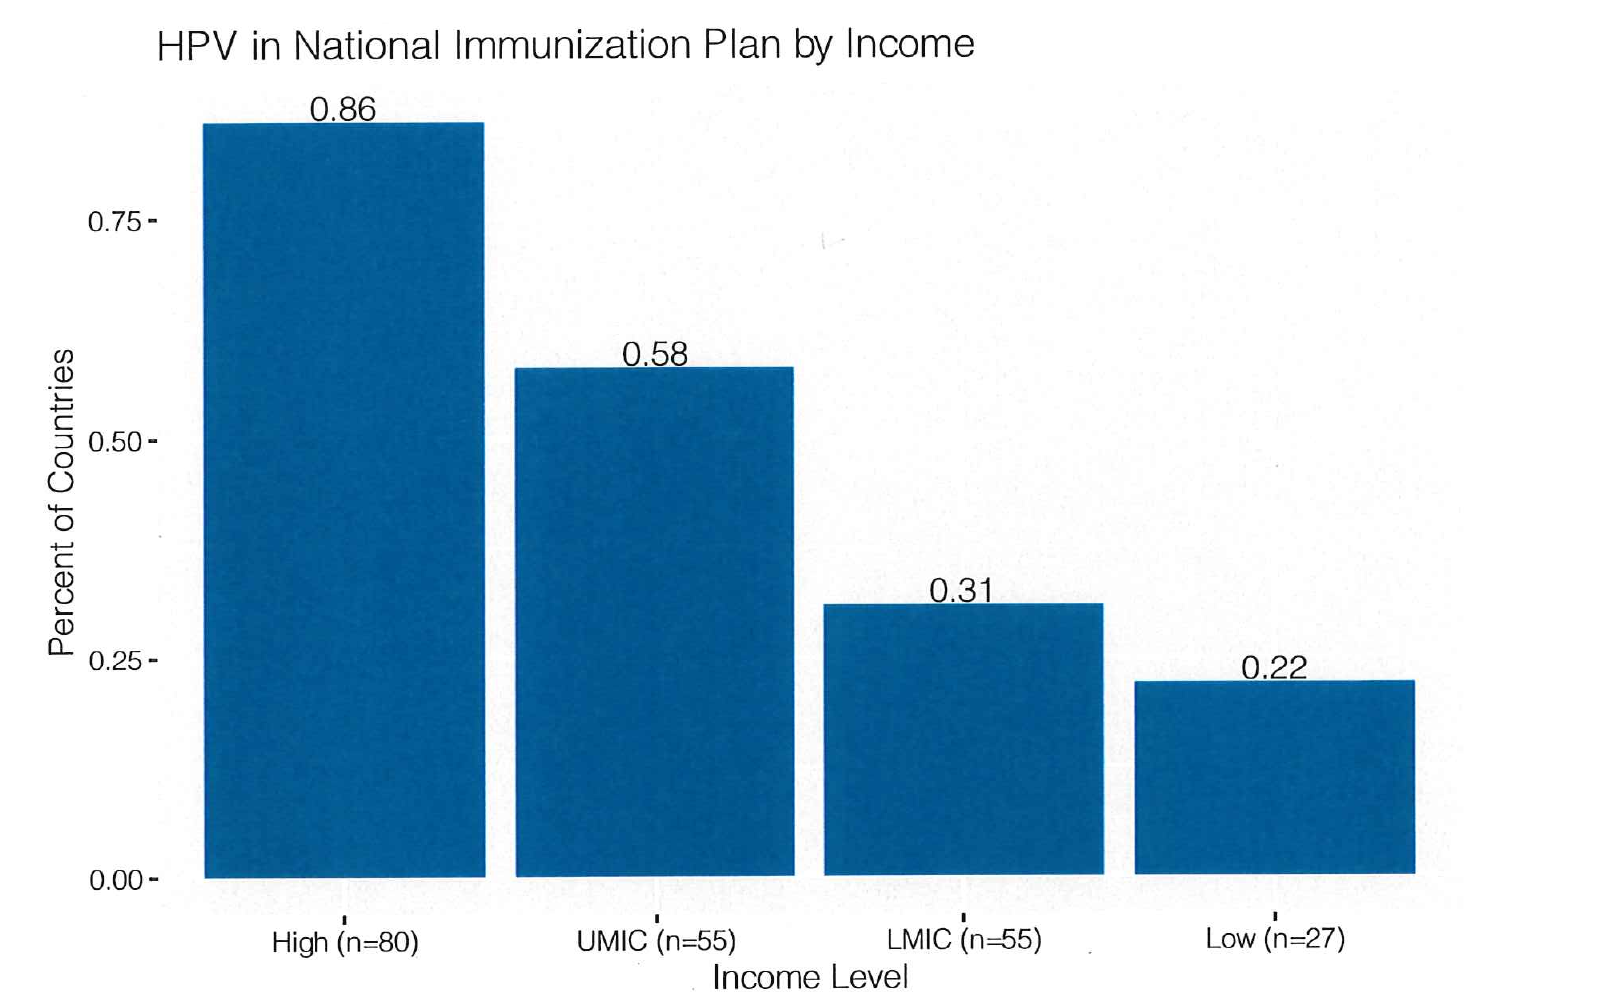
\includegraphics[width=0.86\linewidth,height=\textheight,keepaspectratio]{images/chart_hpv.png}
\end{center}

Let \(H\) be the event a country has HPV in its national immunization
plan and \(L\) be the event that a country is a low-income country.

Find the requested probabilities. If you need additional information to
calculate a probability, state what is needed.

\textbf{10.} \emph{(8 points)} What is \(P(L)\), the probability that a
country is a low income country?

\newpage

\textbf{11.} \emph{(8 points)} What is \(P(H)\), the probability that a
country has HPV in its national immunization plan?

\vspace{3.7in}

\textbf{12.} \emph{(8 points)} What is \(P(H\mid L)\), the conditional
probability that a low income country has HPV in its national
immunization plan?

\vspace{1.25in}

\newpage

\textbf{13.} \emph{(8 points)} What is \(P(L\mid H)\), the conditional
probability that a country is a low income country given that it has HPV
in its national immunization plan?

\vspace{5.9in}

\newpage

\textbf{14.} \emph{(8 points)} Suppose a global health student is
surveying countries about their national immunization plans and takes a
completely random sample of size \(n=10\) from this group of 217
countries. What is the probability that this sample will contain more
than one low-income country?

\vspace{5.9in}

\newpage

\section*{Limits of Human Speed and
Endurance}\label{limits-of-human-speed-and-endurance}
\addcontentsline{toc}{section}{Limits of Human Speed and Endurance}

The New York City Marathon is the largest marathon in the world and
attracts elite runners worldwide (in fact Kenya has more open division
winners than the US!). \emph{OpenIntro Introduction to Modern
Statistics} has an interesting example that shows time to completion (in
hours) of winners in both overall/open divisions of the New York City
marathon from 1970--2020 (the 2021 marathon is in November).

\begin{center}
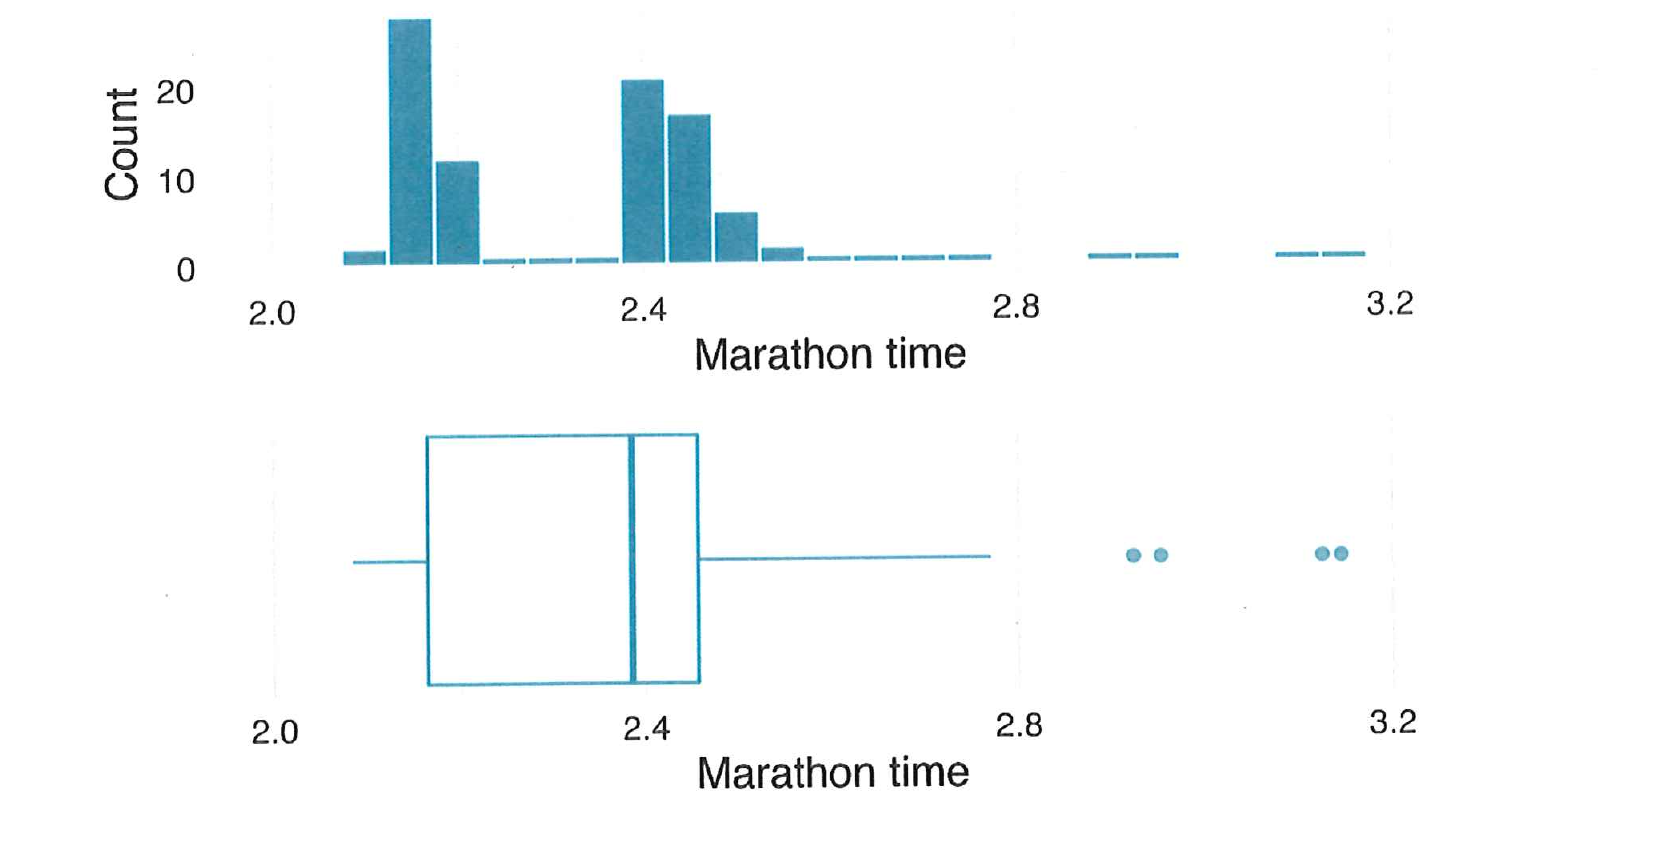
\includegraphics[width=0.91\linewidth,height=\textheight,keepaspectratio]{images/chart_hist_box.png}
\end{center}

\textbf{15.} \emph{(6 points)} What features of the distribution of
winning times are apparent in the histogram but not in the box plot?
Your answer should be based \emph{only} on the features in this
histogram and box plot.

\vspace{1.15in}

\newpage

Below a time series plot of the winning times is provided. Note that
2020 was an anomaly due in part to the marathon's being held as a
virtual event and that the 2012 marathon was not held due to a natural
disaster (Hurricane Sandy).

\begin{center}
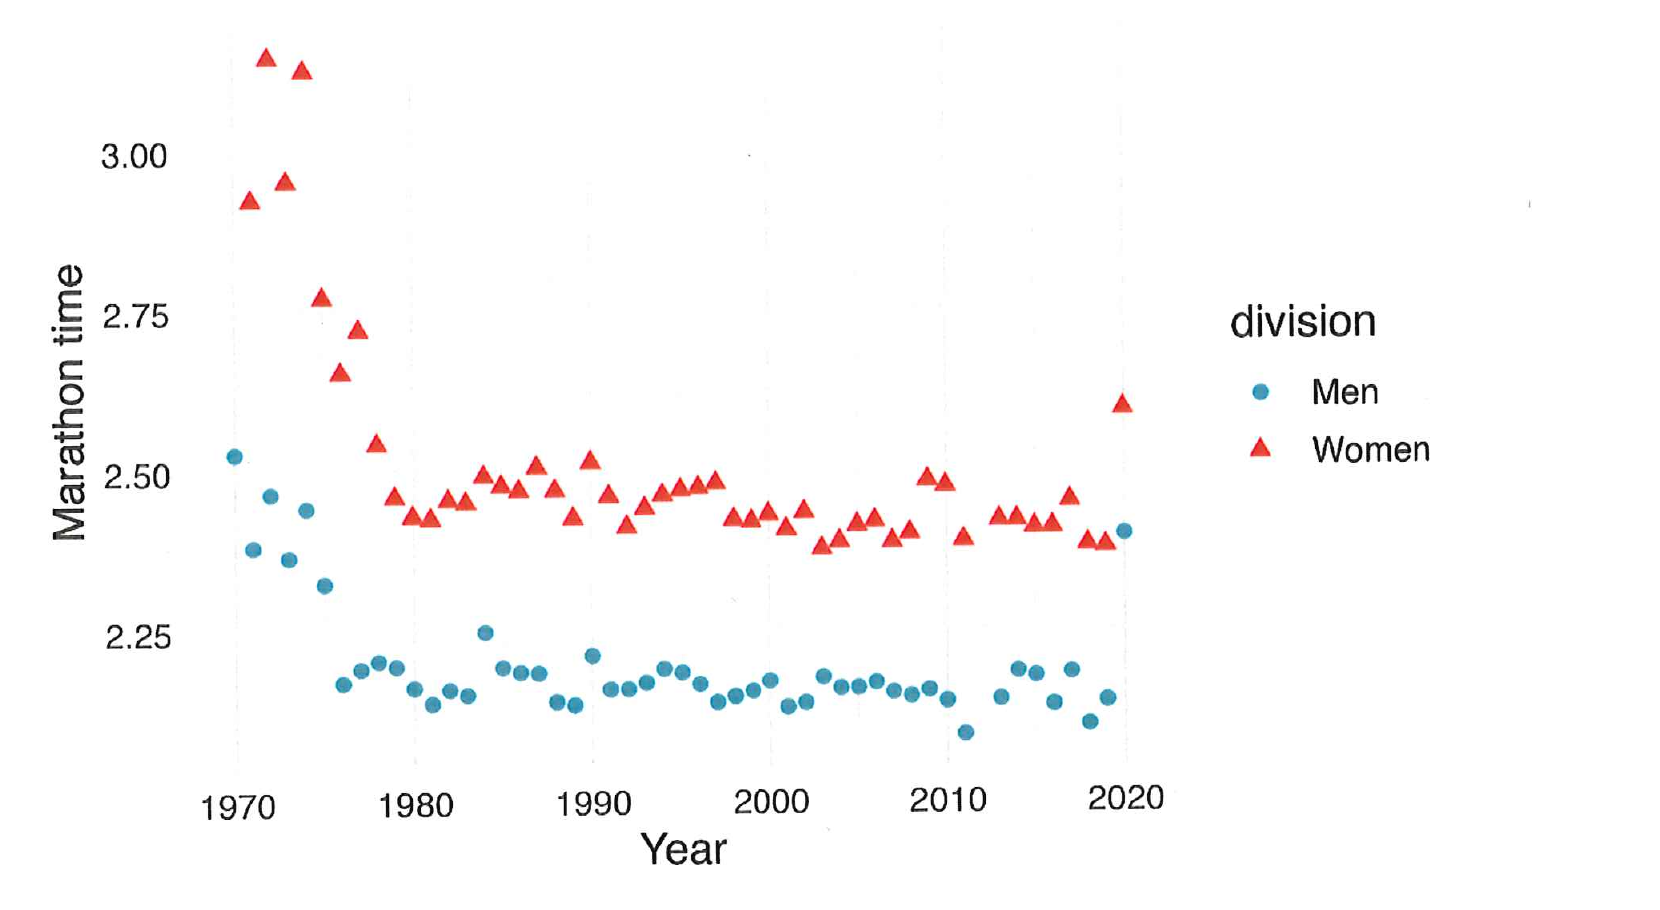
\includegraphics[width=0.87\linewidth,height=\textheight,keepaspectratio]{images/chart_timeseries.png}
\end{center}

\textbf{16.} \emph{(6 points)} What are the two primary advantages of
this time series plot over the histogram and box plot on the previous
page?

\vspace{2in}

\newpage

\textbf{17.} \emph{(6 points)} With this time series plot in mind, what
is the best way to adapt the histogram or box plot on the previous page
to be more informative?

\vspace{5.8in}




\end{document}
